\chapter{Overall Description}

\section{Product perspective}

The system will be developed from scratch and it will completely replace the legacy system. \newline
It is composed by a client part and a server part.
The latter is composed by an application server (CLup Server) where all the logic is located. It also comprehends the web server, the database server and the mail server,
which all communicate with the CLup Server.
It has an interface, the API Manager, which exposes the public CLup API, for the QR validation. It also makes use of an External Map API for querying data about the
distance of the user from the store. This information will be used to inform the user of when leave the current place.\newline
The solution for the client part includes two interfaces based on the user type: the mobile app for the customers and the browser for supermarkets' employee and managers.
There is also the ticketing kiosk which is a tablet with installed a modified version of the mobile app able to print the ticket on place.
\vspace{1em}
\begin{figure}[H]
	\centering
	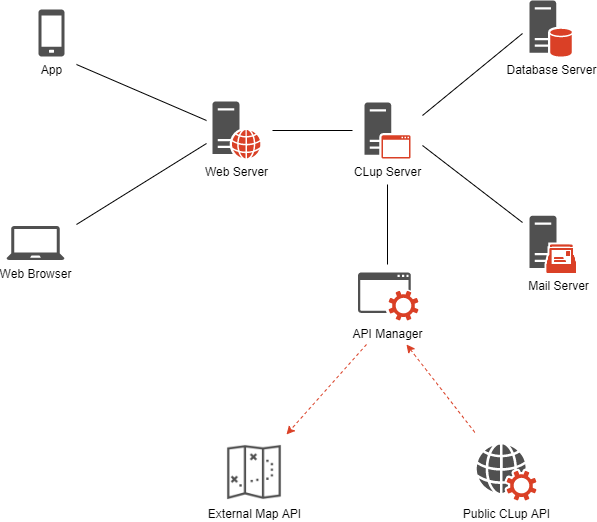
\includegraphics[scale=0.45]{ProdPerspective_Diagram}
	\caption{CLup system diagram.}
\end{figure}

\begin{figure}[H]
	\centering
	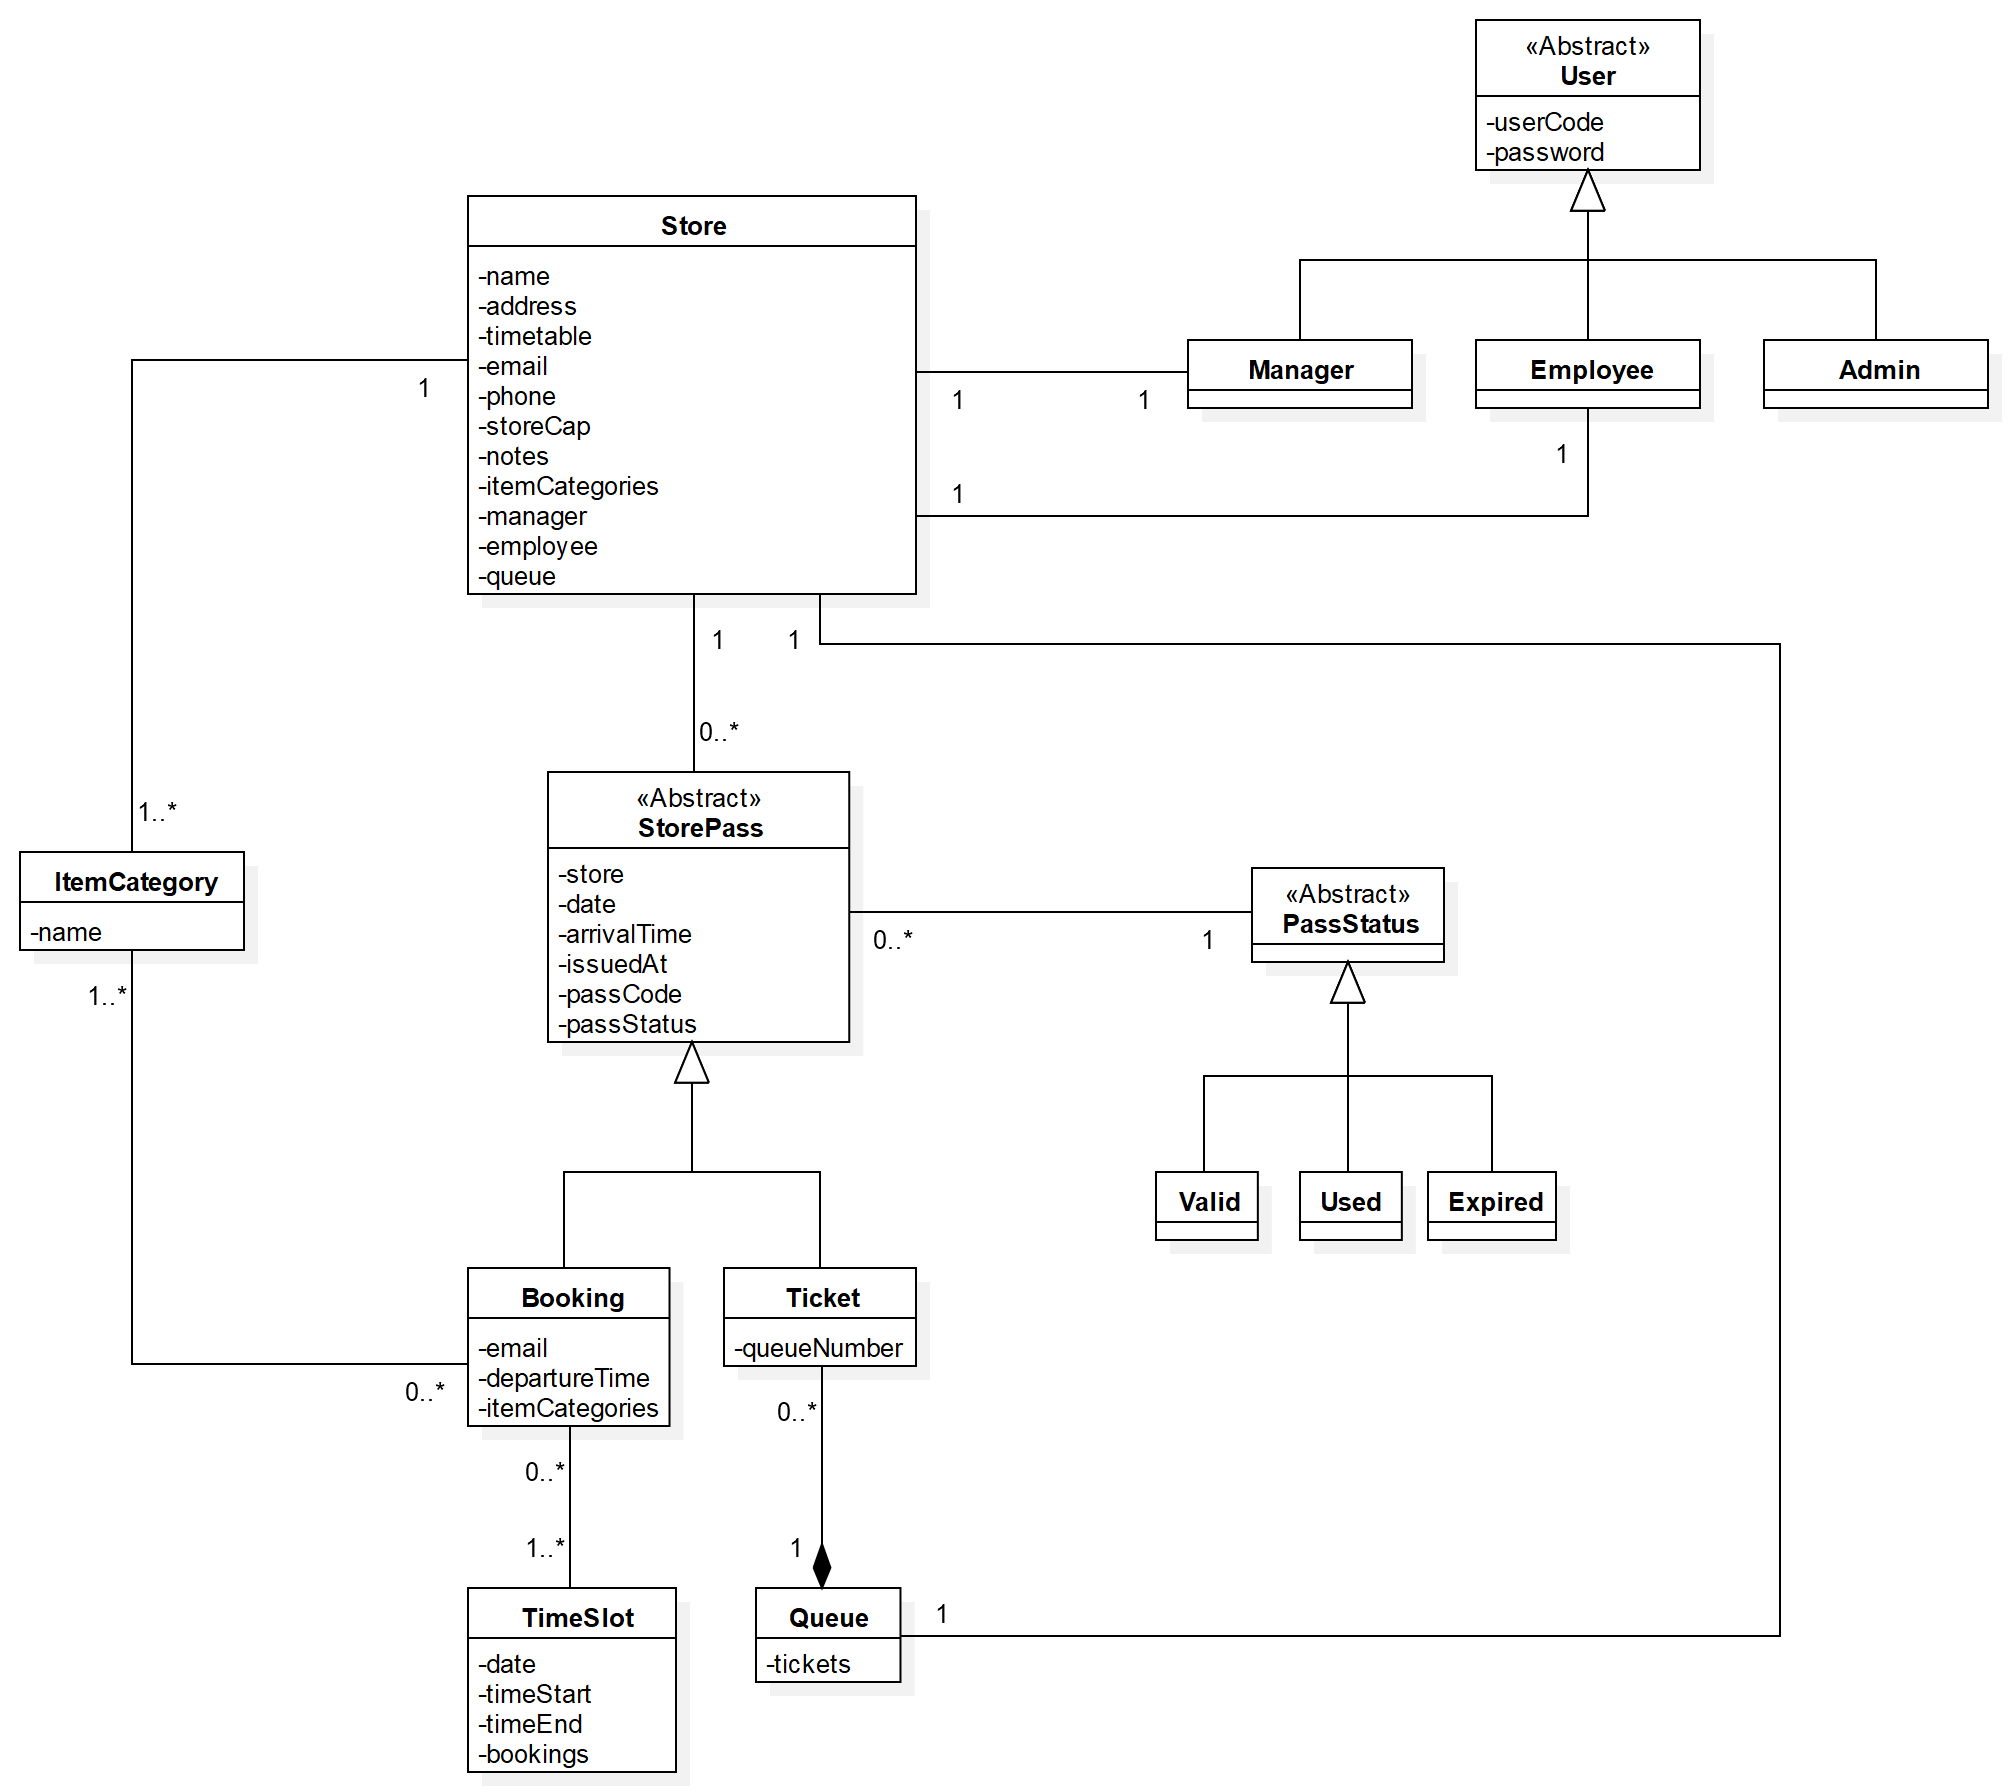
\includegraphics[width=\linewidth]{class_diagram}
	\caption{Class diagram.}
\end{figure}
\section{Product functions}\label{desc:prodFunc}
This section provides a summary of the major functions that the software will perform w.r.t. the goals already described in section \ref{intro:goals}.

\subsection{Queue function}
The main function of \textit{CLup} is to manage queues. A user who wants to do grocery-shopping will join the queue for a specific store through the Mobile App.\newline
Firstly, the user will be asked to select the store in which he desires to line-up.\newline
Then the system will prompt the current size of the queue and an estimate of waiting time. If the user is satisfied with his choice it can subscribe to the queue, operation that will be confirmed by the emission of a ticket. The ticket comprehends a queue number, which identify user's position in the queue, and a QR code, which is used for the ticket validation. At any time the user will be able to check his position in the and the \textit{leave-at-time} (i.e. the time they need to depart from their current position to reach the store); the current position will be retrieved by the GPS of the user device. This requires the GPS service to be enabled, otherwise no time estimation will be shown.

\subsection{Reserve function}
This advanced function allows customers to "book a visit" to the store. Customers are asked to select the store they want to visit. Then they need to fill in a form by indicating:
\begin{itemize}
	\item an \textbf{email address}, which will be needed to send a receipt and memo to the user;
	\item the \textbf{date} of the visit;
	\item the approximate \textbf{expected duration} of the trip;
 	\item the main \textbf{categories of items} they intend to buy;
    \item a \textbf{time slot} chosen from the ones suggested by the system.
\end{itemize}
Every field of the form is mandatory, this means that the user must complete all of them in order to submit the reservation. The time slots will be suggested according to the saturation of the grocery shelves. The system will try to balance the number of people in each section of the store.

In addition, for long-term customers, it also suggests a time inferred by the system based on an analysis of the previous visits.
Customers are also allowed to delete their booking at any time by going to the right section in the Mobile App or by clicking the link sent via email after the reservation.

\subsection{Validation function}
The system provides an API interface that can be queried to allow the validation of QR codes. The process of scanning the QR is to be handled by an external service.\newline
Ticket validation through QR is necessary to speed up the check-in process. At the same time it helps staff to detect the authenticity of tickets brought to them.

\subsection{Dashboard function}
\textit{Customers Line-up} web platform grants supermarkets a way to manage queues and customers inside their stores. In particular, \textbf{upon authentication}, it offers three level of access: \textit{manager-level} and \textit{staff-level} for supermarkets and \textit{admin-level} for CLup administrators.

\begin{itemize}
	\item \textbf{Manager-level}\newline
	With the \textbf{dashboard UI}, store managers have access to tables and data visualizations of their customers visits and behaviours. In particular, they can monitor the number of people in the queue and the ones inside the store. Then, based on those data they can setup the maximum cap of people in the store and in the queue.\newline
	Store managers can view, edit and delete the list of reservations made by the customer.\newline
	Last but not least, they can inspect information about the booked visits at any given time.

	\item \textbf{Staff-level}\newline
	A store employee is able to view data about the number of people in the queue and inside the building. This is needed during the validation of tickets when the check-in staff scans QR and allows customers inside the store.

    \item \textbf{Admin-level}\newline
    An administrator of CLup is able to register new supermarkets and generate the respective credentials to access \textit{manager-level} and \textit{staff-level}.
\end{itemize}

\section{User characteristics}
CLup has three different groups of users:
\begin{itemize}
	\item \textbf{Customers}: they are customers of the supermarket. They can be of all ages and don't necessarily have experience with technology. They can also be elderly
	people who don't have a smartphone at all. For this reason the system should be as easy to use as possible and should provide an alternative way to retrieve a ticket in
	addition to the mobile app.
	\item \textbf{Store managers}: they are the managers of the store. They manage the number of people who can access the store and can monitor the ones that
	are in the supermarket. It is reasonable to assume that they have at least a minimum experience with technology and the use of computer. For this reason the dashboard
	with all the information about customers will be accessible from a web browser.
	\item \textbf{Store employee}: they are the employees of the store. They validate the tickets at the entrance of the store. They could not have experience
	with technology. For this reason the interaction that they should have with the dashboard is reduced to the bare minimum.
    \item \textbf{CLup admin}: an employee of CLup able to register supermarkets and generate their credentials. It can also maintain and update the system. Registration for this kind of users is forbidden and it has to be added directly during the system's installation process.
\end{itemize}

\section{Constraints}
In this topic it is put on paper a general description about considerations, boundaries and items that will limit the system's options.

\subsection{Regulatory policies}
The mobile application requests the user's permission in order to retrieve and use their position at runtime. The email addresses provided when booking through CLup will not be used for commercial purposes or given to third parties.

\subsection{Hardware limitations}
 Here is listed where CLup is available depending on your device. Please note that not all devices are supported.
\begin{itemize}
	\item Mobile App
		\begin{itemize}
			\item iPhones with iOS version 13.5 or above, phones running Android 6 (Marshmallow) or above;
			\item 2G/3G/4G connection or Wi-Fi available;
			\item GPS service.
		\end{itemize}
	\item Web App
		\begin{itemize}
			\item modern web browser like Firefox, Chrome or Safari;
			\item internet connection available.
		\end{itemize}
\end{itemize}

\subsection{Interfaces to other applications}
The proper functioning of the app is strictly subordinated to an external map service which will be accessed via API. This is required to compute travel distance and time for a matrix of origins and destinations (i.e. customer and store position).\newline
In addition, CLup provides an API to be used by an external solution that take charge of the scanning of QR.

A failure in any of the above described services will translate into the inability to use CLup.

\clearpage

\section{Assumptions and Dependencies}
The properties that hold in the analysed world will be listed below.
\subsection{Domain assumptions}
\begin{enumerate}[label=\textbf{D.\arabic*}]
	\item \itemtext{dom:smartphone}{The majority of the customers has a smartphone with internet available.}
	\item \itemtext{dom:categories}{Customers attains to the declared categories of items.}
	\item \itemtext{dom:internetStores}{Stores have an internet contract.}
	\item \itemtext{dom:workingGps}{GPS modules of smartphones are working properly.}
	\item \itemtext{dom:gpsPrecision}{The precision of the GPS modules of smartphones is greater than twenty meters.}
	\item \itemtext{dom:bringSmartphone}{Customers bring with themselves the smartphone that they used to retrieve a ticket or reserve a time slot.}
    \item \itemtext{dom:oneToOneQr}{A ticket or a booked visit is associated with exactly one person.}
    \item \itemtext{dom:custEmail}{Customers who want to book-a-visit have an email address.}
	\item \itemtext{dom:uniqueName}{Stores have unique names.}
	\item \itemtext{dom:employeeEntrance}{Each store has an employee at the entrance which check-in people.}
	\item \itemtext{dom:qrServiceReliable}{External service to scan QRs is reliable and fast.}
	\item \itemtext{dom:qrServiceApi}{External service to scan QRs communicates effectively with CLup APIs.}
	\item \itemtext{dom:storeRegistered}{Store managers have registered their stores in CLup.}
	\item \itemtext{dom:timeArrival}{Customers comply with the arrival time assigned by the mobile app.}
	\item \itemtext{dom:capStores}{Store managers know the maximum capacity of customers in the building.}
   	\item \itemtext{dom:storeKiosk}{Each store has a Self Service Ticketing Kiosk accessible.}
\end{enumerate}

